This section will elaborate on the steps we took to verify the results in the paper. The following steps were taken:

\begin{itemize}
	\item Generate graphs similar to the ones used in the paper.
	\item Implement the proposed algorithms to create optimized SQL queries from the graphs.
	\item Send query to SQL engine and measure the execution time
\end{itemize}

\begin{figure}
	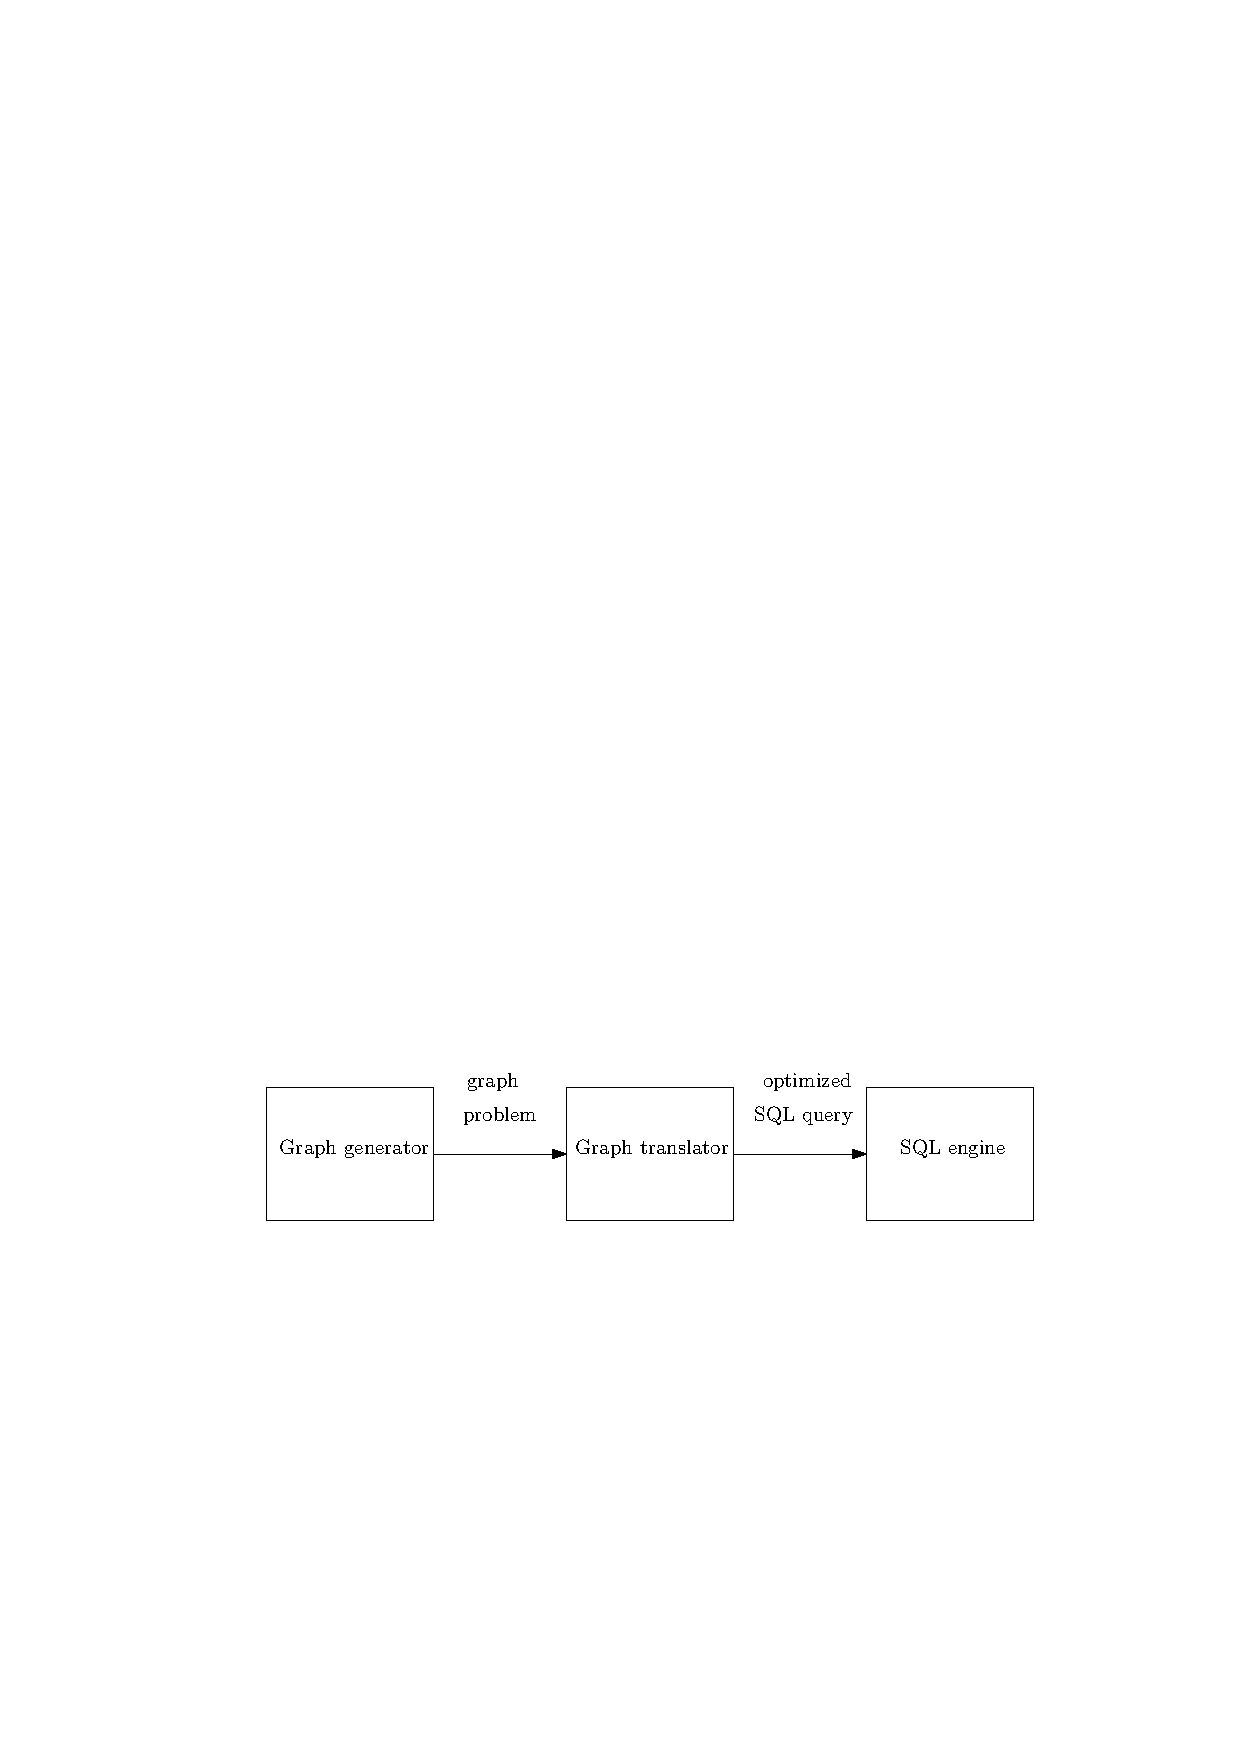
\includegraphics{figures/process.pdf}
	\caption{All steps in the process of verification}
	\label{fig:process}
\end{figure}

\noindent Figure~\ref{fig:process} gives an overview of the process and how the results are passed. The generation and translation of graphs are implemented in Java. The idea is to have a graph generator, which outputs the graph we want to solve. Specifically, we pass a list of graphs, which will be the graphs used for a single experiment, varying in graph order or density. \\

The graph translation part takes the graphs as input and generates SQL queries for the graphs, according to the algorithms proposed in the paper. This part thus returns several SQL queries, in a text-file and can be passed directly to the next part in the process. This is the biggest part of the assignment, so we want worked in parallel on the different algorithms. \\

The queries are passed to a SQL engine. We have chosen to use PostgreSQL, to stay close to the tools that were used in the paper. However, we no longer have access to the older version of Postgres that is used by the authors of the paper, so we choose to use a newer version, namely 9.3.4. The newer version can be more optimized, so we have to take this into account when comparing results. Furthermore, we know that the authors used a Linux cluster of Itanium II, processors with 4GB of memory. We have no access to the cluster and no further details about the hardware are available, so we have to use our own machines.\\

In the next subsection we will elaborate on the different parts of the process and give some more in-depth information we gathered to implement the optimization techniques.

\subsection{Graph Generator}
The graph generator takes a natural number \texttt{amount} as input so that it knows how many graphs it has to generate. Furthermore, it has 6 modes in which it can generate a certain amount of graphs:

\begin{itemize}
	\item Random graphs with a set order, scaling the density up for each of the \texttt{amount} graphs.
	\item Random graphs with a set density, scaling the order up for each of the \text{amount} graphs.
	\item Augmented path graph, with path of length \texttt{n}, thus having \texttt{n} dangling nodes.
	\item Ladder graphs, with \texttt{n} rungs.
	\item Augmented ladder graphs, with \texttt{n} rungs, each having a dangling node at both sides.
	\item Augmented circular ladder graphs, which are the same as Augmented ladder graphs, but the last rung is connected to the first.
\end{itemize}

For the last 4 modes, \texttt{n} scales up for each fo the \texttt{amount} graphs. Using the scaling in size of the graphs, we can precisely mimic the experiments that have been done by the authors of our paper.

\subsection{Query Generator}
The Query Generator will translate the Graphs generated in the previous step, to the optimized queries we want. For the query generator it is important that the edges have a set order during the generation process, since the ordering of the edges can affect the optimization process. For the different techniques, it is important to maintain some information about this ordering with respect to the vertices in the graph.

For the Straightforward approach and further, we need to maintain the first edge in which a vertex has been used. We need this to perform the join in a correct way: each join statement requires us to refer to the attributes that should join, and we can always refer to first time we introduced an attribute to keep the query consistent.

For the Projection pushing approach and further, we need also need to maintain the last edge in which a vertex is used. When a vertex will no longer be used, when we join the edges in the specific order, we can project it out.

Bucket elimination requires a far more complex approach. Although we did not get it working in the given time, we still provide information about it in the next section.

\subsection{Bucket elimination}
In this section we will give all the research we have done into bucket elimination, to give an overview of the information we needed to implement this technique.\\

Bucket elimination represents the query as a join-expression tree, instead of a linear projection-join sequence. A sequence in the vertices is determined and then buckets are formed that can reproduce query with a tree-like join structure in its subqueries. The steps in the bucket elimination process are as follows:

\begin{enumerate}
	\item Create a benificial order for the vertices
	\item Create a bucket per vertex and divide the edges over the buckets in a benificial way
	\item Consider the buckets one at a time, in the order of the vertices
	\item Create a subquery per bucket and put it in a not yet considered bucket, in a benificial way
	\item The last bucket will provide the full query.
\end{enumerate}

What is left is to explain what order we want for the vertices, how the edges are put in the buckets and in what bucket we put a produced subquery. 

\paragraph{Preparation for Bucket Elimination Algorithm execution}
We start by explaining the Maximum Cardinality Search algorithm, which will give us a good sequence of vertices we can use. Algorithm~\ref{alg:mcs} shows the pseudocode for finding the MSC order of the vertices.

\begin{algorithm}
\caption{MCS}\label{alg:mcs}
\begin{algorithmic}[1]
\Procedure{MSC}{$G(V, E)$}
    \For{$i\gets 0, \#V$}
	\State $V[i].label \gets 0$
    \EndFor
    \For{$p \gets 0, \#V$}
	\State Pick the first vertex \texttt{v} which has the highest label and $V[v] == null$
	\Comment{First round pick a random vertex, since all have no position}
            \State $V[v].position = p$
            \ForAll{$edge \gets E$} 
		\If{$edge(v, u)$ $or$ $edge(u,v)$}\Comment{Find edges that involve the chosen v}
                		\State $V[u].label++$
		\EndIf
            \EndFor
    \EndFor
\EndProcedure
\end{algorithmic}
\end{algorithm}

\paragraph{Bucket Elimination Algorithm Execution}
Given the MCS order of the vertices we create a bucket for each vertex and now we consider these buckets iteratively, from the last to the first and eliminate the latest bucket every time (bottom up method). The Bucket of the vertex $v_i$ stores:
\begin{itemize}
\item Every edge, which contains vertex $v_i$. $edge(v_i,X) edge(X,v_i)$
\item Every query regarding vertex $v_i$
\end{itemize}
\noindent During these iterations, inside the considering bucket there are several relations, where there is a specific attribute, iconic for this bucket, in all these relations. For all these relations, their join is computed and attributes are projected out, if they do not belong to the target schema, which we want in the end. For this reason, each bucket has live vertices. These are:
\begin{itemize}
\item Every vertex, which appear inside the edges of the bucket. $edge(v_i,LiveVertex) edge(LiveVertex,v_i )$
\item Every vertex, which appear inside SELECT section of bucket’s queries
\end{itemize}
So, as mentioned above, we process these buckets in descending order according to MCS order in the following way. A bucket is processed by this way:

\begin{enumerate}
\item Create the following query \\
\underline{SELECT} all the \emph{live vertices} of the bucket \\
\underline{FROM} all \emph{edges} and \emph{queries} of the bucket\\
\underline{JOINing} them \\
\underline{ON} \emph{straightforward} approach conditions
\item Find the destination of the above query between the live vertices of the bucket. This means that we have to find the maximal vertex in query's  SELECT section. With the term maximal, we indicate the vertex with the position which is closer to the first one according the MCS order. 
\item Move the query, which is created during the first step, to chosen vertex' bucket and then eliminate the processed bucket.
\end{enumerate}

When we reach the final bucket we will not execute the $2^{nd}$ and the $3^{rd}$ step, but we will change the SELECT section, with SELECTing only one vertex in Boolean case or SELECTing the free vertices in non-Boolean case.

The result can be empty, and in that case the result of the whole query is empty. If it is not empty, we place the resulting relation in the highest bucket, which has an attribute in the joined relation that is iconic for the bucket. If this process terminates with there still being a relation in the last bucket, we have found the non-empty result of our query.

\subsection{Connection with PostgreSQL}
We use a Java library to send the generated queries directly to the PostgreSQL database. However, we need tables in the database that have the correct format. Therefore, we made a Table generator, which generates the CREATE statements for the required tables. If we choose to have a maximum order, we can number the vertices from 0 to $order - 1$, and generate a table with the 6  colour-combination entries, for each couple of vertices.
